% Chapter Template

\chapter{Introducción específica} % Main chapter title

\label{Chapter2} % Change X to a consecutive number; for referencing this chapter elsewhere, use \ref{ChapterX}

%----------------------------------------------------------------------------------------
%	SECTION 1
%----------------------------------------------------------------------------------------
En este capítulo se presentarán los módulos principales del equipo dip coater propuesto y las tecnologías asociadas a cada uno ellos. 
\section{Elección de las tecnologías}

De la experiencia de uso del cliente con diferentes equipos dip coater se desprenden a continuación una serie de requerimientos funcionales respecto a los movimientos que se tienen en cuenta para la elección de las tecnologías: 

\begin{enumerate}
			\item El sistema debe permitir que el usuario pueda configurar en un programa variables de desplazamiento y tiempos de espera.
			\item El sistema debe contar con un rango de velocidades de desplazamiento de muestra configurables entre [1- 1000 \si{\milli\meter\per\minute} ]. 
			\item El sistema debe contar con un rango de aceleraciones de desplazamiento de muestra configurables entre [1000 - 15000 \si{\meter\per\square\minute}].
		
\end{enumerate}
	
Como se describió en el sección \ref{sec:dip coating} para lograr \textit{film} sin daños estructural es importante controlar con exactitud las variables de movimiento. Para entender el impacto de un control correcto se tuvo en cuenta la publicación \cite{paper_galo}  en donde se describe la técnica dip coating como un proceso dinámico complejo difícil de modelar, debido a los gradientes de concentración y viscosidad inducidos por la evaporación de la solución. Sin embargo, es una técnica muy difundida porque es simple y proporciona una excelente reproducibilidad. 

Existen entonces modelos matemáticos basados en la mecánica newtoniana que no tienen en cuenta la evaporación de las soluciones y requieren varias suposiciones y simplificaciones. En estos modelos llegar a la predicción del espesor depende de la densidad, la tensión superficial y la viscosidad del fluido. El problema con este modelo es que la mayoría de las soluciones utilizadas son fluidos no-newtonianos, es decir en donde el solvente de la solución se va evaparonado en simultáneo con la extracción de la muestra induciendo una modificación en la densidad, tensión superficial y viscosidad del fluido. 


La publicación se basa entonces en  un estudio semi-experimental sobre varias soluciones químicas para predecir el espesor final de la película. Tiene en cuenta dos modelos matemáticos, un modelo de capilaridad asociado a extracciones en velocidades bajas y otro modelo de evaporacion asociado a velocidades altas. 

Se observa en la figura \ref{fig:paper_galo} la variacion de los espesores fabricados respecto a la velocidad utilizada, también se puede observar como se relacionan los diferentes modelos. 

\begin{figure}[htpb]
\centering 
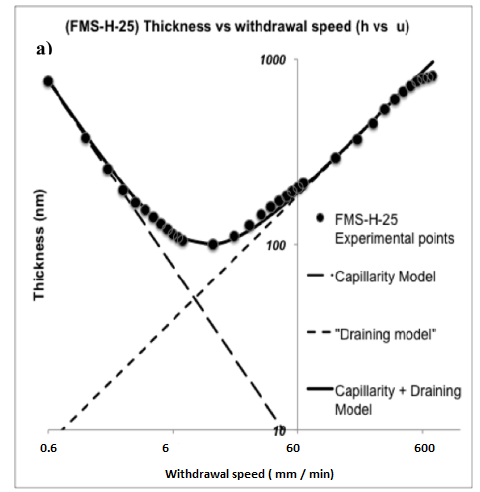
\includegraphics[width=0.6\textwidth]{./Figures/paper_galo.png}
\caption{Espesor vs extracción. Imagen tomada de publicación.}
\label{fig:paper_galo}
\end{figure}

Los resultados del experimento concluyen en que existe linealidad  en la relación de espesor respecto la velocidad de extracción entre \SI{60}{\milli\meter\per\minute} y \SI{600}{\milli\meter\per\minute} . En donde el fenómeno se puede explicar por el modelo de evaporación.

La importancia de estos resultados es que el rango de velocidades quedá incluido dentro de los requerimientos de nuestro equipo. Cabe destacar que todos los experimentos en la publicación fueron a  velocidad constante. De las reuniones con el cliente y del interés de trabajar en la frontera de la ciencia surgió la necesitad de poder darle al usuario la posibilidad de realizar experimentos a velocidad y aceleración controlada.  Esto último es una cualidad que diferencia a nuestro equipo de todos los equipos comerciales relevados. 
  

\section{Movimientos controlados}
\subsection{Circuitos Integrados Trinamic}

Del estudio del proceso dip-coating y teniendo en cuenta la importancia del control preciso necesario para el desarrollo del experimento se propone entonces trabajar con el fabricante de circuitos integrados \textit{TRINAMIC Motion Control}\citep{3_web_trinamic}. Como su nombre lo indica Trinamic se dedica a fabricar circuitos integrados para el control de diferentes tipos de motores, su lema se basa en convertir señales digitales de control en movimientos presisos. Tiene una trayectoria de veinte años en la industria y actualmente fue adquirida por la companía Analog Devices.
De las reuniones con el cliente y el estudio se definen entonces los siguintes requerimientos:
			
\begin{itemize}
\item El equipo deberá contar para realizar los movimientos con un motor paso a paso Nema 17.
\item Se utilizará un driver de motor de la marca TRINAMIC.
\end{itemize}

Cabe destacar que los integrados fabricados por la empresa Trinamic se utilizan en diversas aplicaciones en donde la presición importa, como por ejemplo impresion 3d, automatización industrial, robótica, equipos de laboratorio médico entre otras.
Cuenta con una amplia gama de productos que se diferencian en general por el tipo de motor que se quiera accionar. En nuestro caso como ya tenemos defino la utilización del motor paso a paso vamos a trabajar con el ultimó integrado diseñado para dicho fin, el mismo será el TMC5130. 
  
Todos los integrados requieren ser configurados para su correcta utilización, es por eso que la empresa a demás de proveer los circuitos integrados, ofrecen placas de desarrollo que permiten dar los primeros pasos respecto a laconfiguración del los CI. La placa de desarrollo para este integrado es la \textit{TMC5130-Eval Evaluation Board}, la misma esta conectada a otra placa general compatible con diferentes placas de evaluación con la cual a través de un software provisto por el fabricante podemos realizar trabajos de configuración en el circuito integrado y encontrar los parametros que mejor se adaptan al motor que utilizaremos y a la carga que el mismo tenga aplicado. A continuación en la figura \ref{fig:tmc5130_placa} podemos observar a izquierda la placa Startrampe  que se conecta entre la computadora y la placa de evaluacion del circuito integrado TMC5130 que se observa a derecha.

\begin{figure}[h]
\centering 
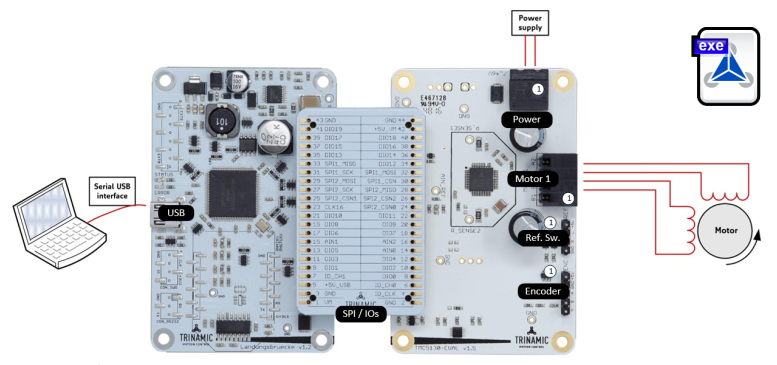
\includegraphics[width=0.9\textwidth]{./Figures/tmc5130_placa.png}
\caption{Placa de desarrollo Startrampe + placa de evaluación TMC5130.}
\label{fig:tmc5130_placa}
\end{figure}

  
\subsection{Driver TMC5130}

El driver TMC5130 es un driver que permite operar motores bipolares de dos fases, comúnmente conocidos como motores paso a paso. El circuito integrado incorpora la respectiva estapa de potencia a traves de tecnología MOSFET que le permite manejar corrientes de hasta 2 amperios por fase.
A continuación describiremos los módulos principales del CI y en el capítulo \ref{Chapter3} se darán mas detalles de la configuración de los módulos implementados en nuestro equipo.

Podemos observar en la figura \ref{fig:tmc5130_diagrama} el diagrama en bloque del CI. 

\begin{figure}[h]
\centering 
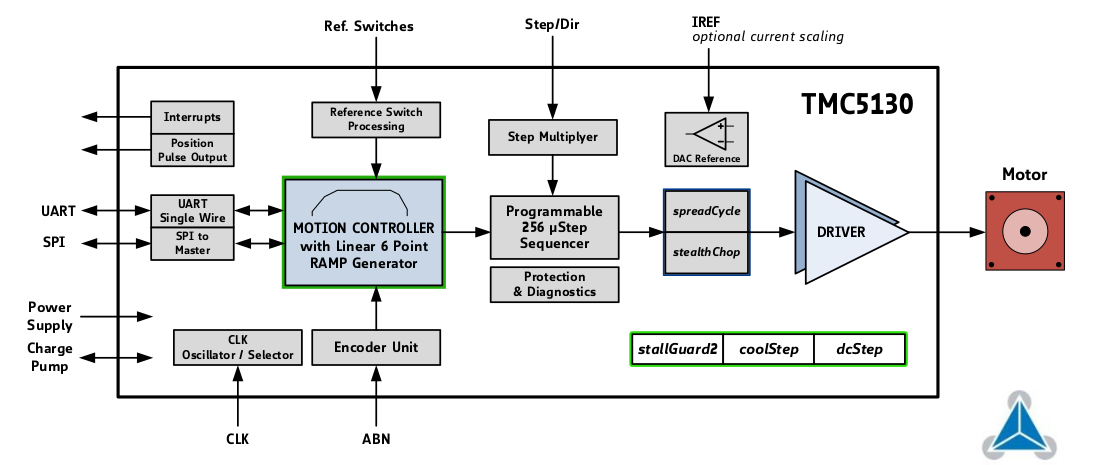
\includegraphics[width=1\textwidth]{./Figures/tmc5130_diagrama.png}
\caption{Diagrama en bloque TMC5130.}
\label{fig:tmc5130_diagrama}
\end{figure}

La comunicación con el CI se puede establecer a través del protocolo UART \textit{Universal Asynchronous Receiver-Transmitter} o SPI \textit{Serial Peripheral Interface},en el caso de nuestro equipo utilizaremos la comunicación SPI  .Una característica muy importante a destacar es la posibilidad de programar micropasos. Los pasos estan relacionados con las fases  y con la cantidad de dientes que tiene el rotor y estator del motor. Un paso es el mínimo movimiento que el motor puede hacer. Un motor paso a paso como su nombre lo indica realiza movimientos a través de pasos sucesivo, por ejemplo es común contar con algún motor en donde la especificación dice que el paso es de \ang{1.8}, esto signifíca que por cada vuelta de motor \ang{360} el motor realizará 200 pasos.

Una funcionalidad que incorpora este CI es incrementar la cantidad de pasos, el fabricante los denomina micropasos, y se pueden llegar a generar hasta un máximo de 256 micropasos por cada paso del motor. Siguiendo con el ejemplo recién presentado, para un motor de paso \ang{1.8} tendríamos en total 51200 micropasos.


Otra funcionalidad que se utilizará es \textit{Stallguard2}, una función de alta presición que mide la fuerza contraelectromotriz generada en la bobinas del motor por cambios en de carga en el eje del motor. Como se observa en la figura \ref{fig:tmc5130_stallGuard2} el valor de stallguard se decrementa linealmente a medida que la carga en el eje del motor aumenta. En nuestro caso se utilizará esta funcionalidad para realizar un \textit{homing} inicial en el equipo, es decir para encontrar una posición inicial que sirva como referencia para todos los desplazamientos posteriores.
     
\begin{figure}[h]
\centering 
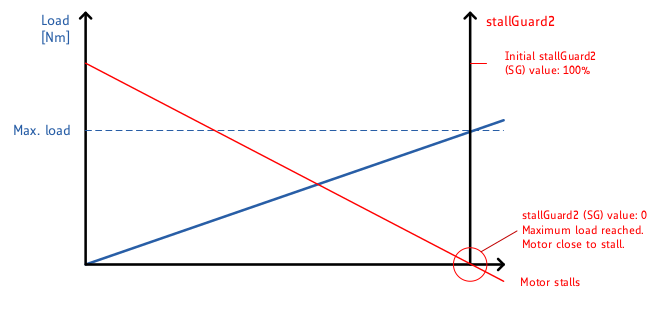
\includegraphics[width=0.9\textwidth]{./Figures/tmc5130_stallguard2.png}
\caption{Función stallGuard2.}
\label{fig:tmc5130_stallGuard2}
\end{figure}

También se utilizará \textit{coolStep}, una función que a través de mediciones de carga en el eje del motor adapta automáticamente la corriente suministradá en las bobinas, cuyo efecto reduce la energía según hojas de datos hasta un \SI{75}{\percent} como puede observarse en la figura \ref{fig:tmc5130_coolStep}. Incluso en aplicaciones en donde la carga es constante como es el caso de nuestro equipo el efecto de ahorro energético es considerable.

\begin{figure}[h]
\centering 
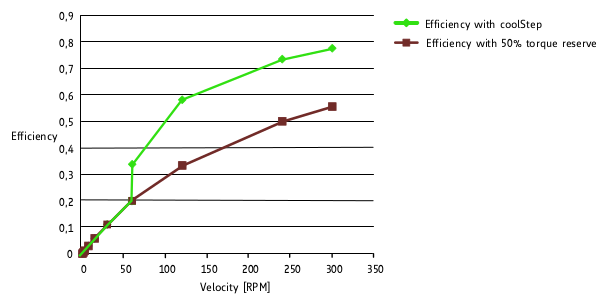
\includegraphics[width=0.9\textwidth]{./Figures/tmc5130_coolstep.png}
\caption{Función coolStep.}
\label{fig:tmc5130_coolStep}
\end{figure}

Por último en cuanto a funcionalidades se analizará la función \textit{dcStep},que es un modo de conmutación automática que ajusta la velocidad del motor en caso de existir cierta sobrecarga del eje, es decir que si no puede mover la carga acoplada al eje con la velocidad establecida se ajusta a una velocidad menor para poder seguir en movimiento y no detenerse por completo. 


En el cápitulo \ref{Chapter3} se darán mas detalles de las configurariones particulares con las que cuenta el equipo.

\section{Interfaz de usuario}

Respecto a la interfaz usuario-máquina surgió de reuniones con el cliente que se esparabá contar con una interfaz moderna de configuración. También se esperaba poder configurar el equipo a pie de máquina evitando estar conectado con una computadora como única opción. Dando así lugar al siguiente requerimiento:
\begin{itemize}
\item La configuración de la máquina debe poder realizarse a través de una pantalla touch.	
\end{itemize} 

Luego de una investigación de mercado sobre los diferentes fabricantes de pantallas táctiles y teneniendo en cuenta la relación costo-calidad se eligió al fabricante de pantallas STONE \citep{web_stone}. La pantalla seleccionada es la STWI043WT/N-01 de 4.3 pulgadas cuyas especificaciones se detallan en la siguiente tabla \ref{tab:tabla_stone} y se compararán con su modelo predesesor:


\begin{table}[h]
	\centering
	\caption[compatación stone]{comparación de pantallas touch stone 4.3 inch}
	\begin{tabular}{l c c}    
		\toprule
		\textbf{}     & \textbf{STWI043WT} & \textbf{STVI043WT}\\
		\midrule
		CPU 			& 	Cortex A8         & 	CortexM4 \\		
		Refresh Rate    & 	1G Hz         & 	200MHz\\
		Image format  	& 	png,bmp,jpg,svg,gif          & 	bmp,jpg \\
		TFT Panel  		& 	Innolux original          & 	Innolux assembly \\
		Flash  			& 	256MB          & 	128MB \\
		Color  			& 	18 bit          & 	16 bit  \\
		PCB 			& 	2.0mm black, ROHS standard          & 	1.6mm green \\
		Font 			& 	TTF vector font file, more sharp and smooth          & 	Dotmatrix font \\
		Interface 		& 	RS232/RS422/RS485/TTL           & 	RS232/RS485/TTL \\
		\bottomrule
		\hline
	\end{tabular}
	\label{tab:tabla_stone}
\end{table}





\begin{figure}[h]
\centering 
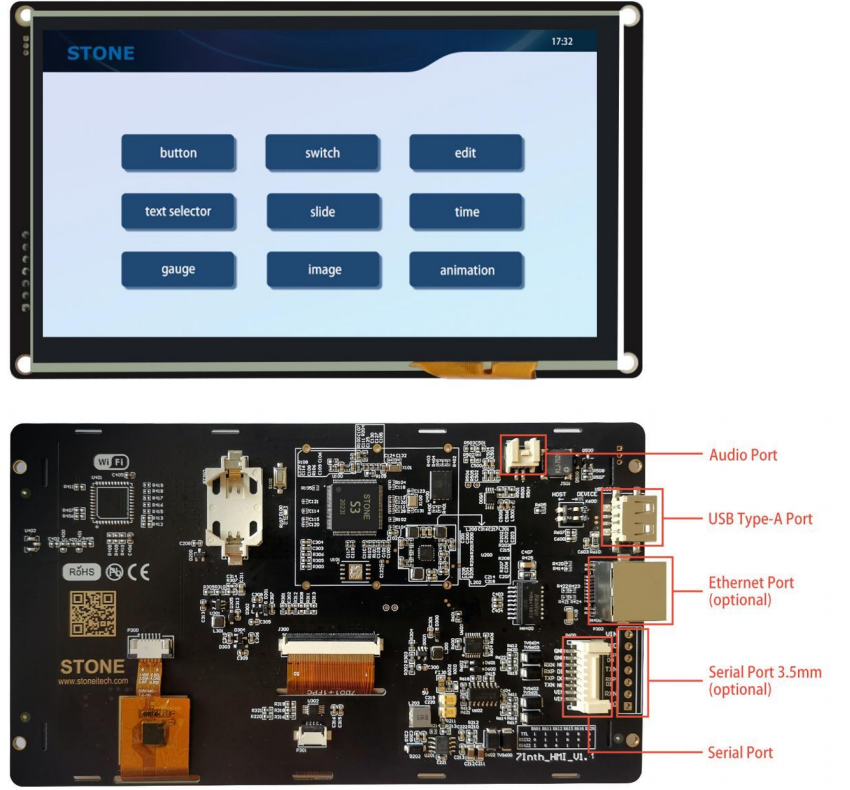
\includegraphics[width=0.9\textwidth]{./Figures/stone.png}
\caption{Display táctil Stone.}
\label{fig:equipo}
\end{figure}


\section{Equipo propuesto}

Como se observa en la figura \ref{fig:equipo}, el equipo dip coater que se desarrollará estará compuesto por: 

\begin{figure}[h]
\centering 
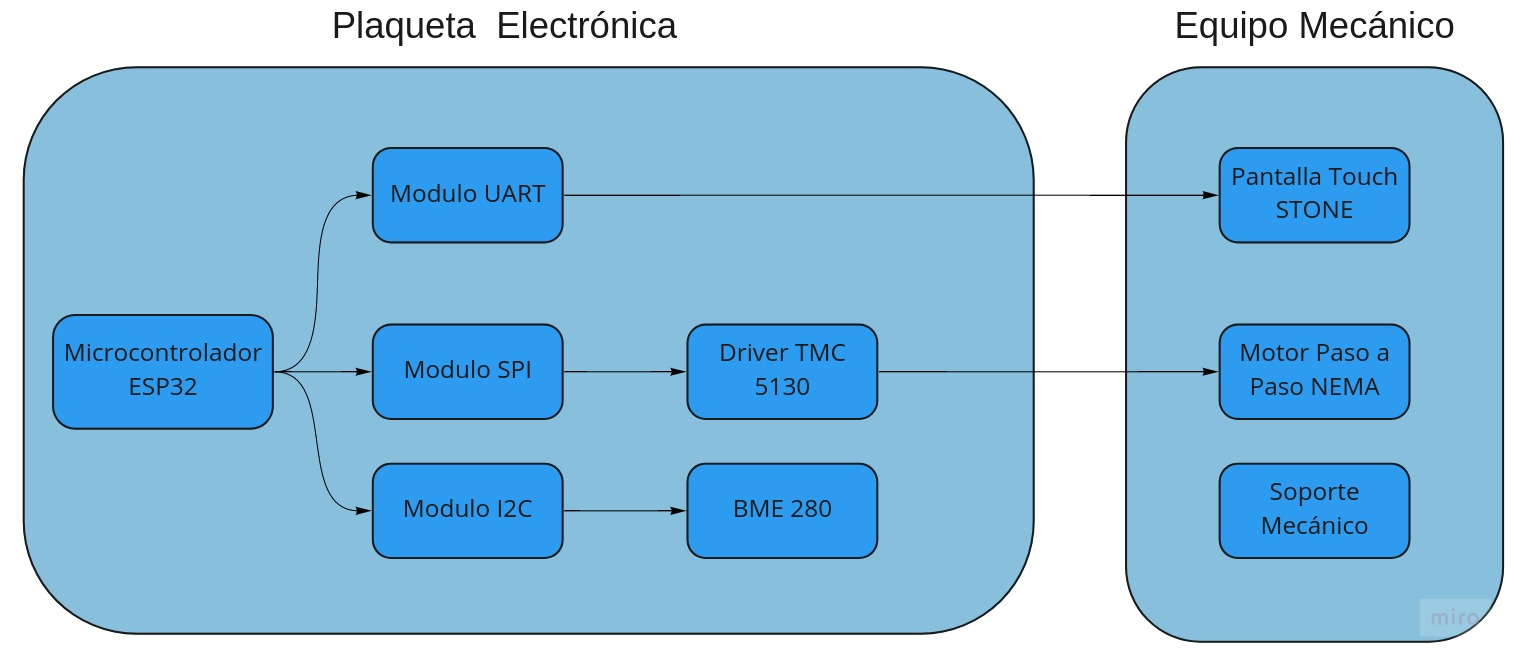
\includegraphics[width=0.9\textwidth]{./Figures/equipo.png}
\caption{Módulos principales del firmware.}
\label{fig:equipo}
\end{figure}
\vspace{25px}


\begin{itemize}
\item Microcontrolador ESP32. 
\item Periféricos principales (GPIOs UART SPI I2C). 
\item Driver de motor paso a paso TRINAMIC  TMC5130.
\item Pantalla táctil STONE. 
\end{itemize}


